\chapter{Exploitation et préparation}

% Indications :
%  Mise en production, déploiement, formation, support et exploitation proprement dite....
% 
% Bon courage ;-)

\section{Installation des librairies et drivers}
Afin d'assurer le bon fonctionnement de l'application, cette dernière requiert que soient présents les packages suivants (dans une version égale ou supérieure à celle précisée)~:
Les éléments nécessaires à la première mise en service sont fournis dans le livrable initial.
\\

\begin{tabularx}{\linewidth}{X X}
	\toprule
	Microsoft Windows	& GNU/Linux		\\
	\midrule
	Windows 7			&				\\
	MinGW 4.8.1 (TMD)	&				\\
	Qt 5.2.1			& Qt 5.2.1		\\
	QMySQL 5.6.16		& QMySQL 5.6.16				\\
	\bottomrule
\end{tabularx}

\subsection{Création du pilote MySQL pour Qt5}
Cette section précise comment créer le pilote MySQL pour Qt5 en utilisant MinGW.
La rédaction de cette dernière a été motivée par le fait que le pilote en question n'est malheureusement pas fournit par défaut dans le framework Qt.


\paragraph{Installation du framework Qt}
L'installation des composants par défaut convient très bien, mais il est tout à fait possible de procéder à une installation complète. Sélectionner le répertoire racine d'installation du framework (ici C:). À terme, Qt est alors installé, ici dans le répertoire C:/Qt/Qt5.2.1.
\\
Ensuite, extraire les sources Qt dans un répertoire temporaire de son choix, puis copier le dossier \textit{qt-everywhere-opensource-src-5.2.1} ainsi obtenu dans le répertoire \textit{C:/Qt/Qt5.2.1/} et le renommer \textit{sources}.
\\
En fin de manipulation, le framework Qt est installé dans le répertoire C:/Qt/Qt5.2.1/ et les sources présentes dans C:/Qt/Qt5.2.1/sources/.

\paragraph{Installation du driver QMySQL}

\subparagraph{Installation sous Linux }
 Vous avez besoin des fichiers d'en-tête de MySQL ainsi que la bibliothèque partagée \textit{libmysqlclient.so}. Selon votre distribution Linux, vous devez peut-être installer un paquet qui est généralement appelé "mysql-dev". 
\\ Dites à \textbf{qmake} où trouver les fichiers d'en-tête de MySQL et les bibliothèques partagées (ici, on suppose que MySQL est installé dans /usr/local) et lancez make : 
\begin{lstlisting}
cd $QTDIR/src/plugins/sqldrivers/mysql
qmake "INCLUDEPATH+=/usr/local/include" "LIBS+=-L/usr/local/lib -lmysqlclient_r" mysql.pro
make
\end{lstlisting}
Après l'installation de Qt, vous devez également installer le plugin dans l'emplacement standard :
\begin{lstlisting}
cd $QTDIR/src/plugins/sqldrivers/mysql
make install
\end{lstlisting}

\subparagraph{Installation sous Windows}
Vous devez obtenir les fichiers d'installation de MySQL. Exécutez \textit{Setup.exe} et sélectionnez "Installation personnalisée". Installez le module "Libs \& Inclure les fichiers". Construire le plugin comme suit (ici on suppose que MySQL est installé dans C:\textbackslash MySQL) : \\
\begin{lstlisting}
cd %QTDIR%\src\plugins\sqldrivers\mysql
qmake "INCLUDEPATH+=C:/MySQL/include" "LIBS+=C:/MYSQL/MySQL Server 5.6.16/lib/opt/libmysql.lib" mysql.pro
nmake
\end{lstlisting}

Si vous n'utilisez pas un compilateur Microsoft, remplacer \textbf{nmake} avec \textbf{make} dans la ligne ci-dessus.
\\


\paragraph{Construction \& déploiement}
Ouvrir le terminal de commande de Qt.
Ce dernier fonctionne comme n'importe quel terminal à ceci prêt qu'il définit par défaut toutes les variables d'environnement Qt nécessaires.
Il s'ouvre sur le répertoire Qt.
\\
Exécuter les commandes suivantes~:

% XXX @mj : essaie de push des fichiers qui compilent ...

\begin{lstlisting}[language=Bash, escapechar=$]
set mysql=C:\\PROGRA~2\\MySQL\\MYSQLS~1.6
cd C:\Qt\Qt5.2.1\sources\qtbase\src\plugins\sqldrivers\mysql\
qmake "INCLUDEPATH+=%mysql%\\include" "LIBS+=%mysql%\\lib\\libmysql.lib" -o Makefile mysql.pro
mingw32-make
\end{lstlisting}
Après construction réussie (et sans erreur), des fichiers seront produits dans \\ C:/Qt/Qt5.2.1/sources/qtbase/plugins/sqldrivers, que sont~:
\begin{enumerate}
	\item libqsqlmysql.a~;
	\item libqsqlmysqld.a~;
	\item qsqlmysql.dll~;
	\item qsqlmysqld.dll.
\end{enumerate}
\begin{lstlisting}[language=Bash, escapechar=$]
For .dll files, move them to C:\Qt\QT5.1.1\5.1.1\mingw48_32\plugins\sqldrivers.

For .a files, move them to C:\Qt\Qt5.1.1\5.1.1\mingw48_32\lib

Also, copy libmysql.dll from %mysql%\lib to C:\Windows
Testing

To use the driver, don't forget to add QT += sql to project file, else it don't work.

Check which drivers are available by this code:

C++
#include <QtCore/QCoreApplication> #include <QtSql> int main() { QCoreApplication a(argc, argv); aDebug() << QSqlDatabase::drivers(); return a.exec(); }
1
2
3
4
5
6
7
8
	
#include <QtCore/QCoreApplication>
#include <QtSql>
 
int main() {
    QCoreApplication a(argc, argv);
    aDebug() << QSqlDatabase::drivers();
    return a.exec();
}

\end{lstlisting}

 \section{Procédure de génération de la base de données}
 Cette section présente la suite logicielle utilisée pour la génération des bases de données de notre programme. 
 Pour ce faire, nous avons utilisé l'outil JMerise permettant de conceptualiser et d'établir les relations au sein de notre MCD.
 
 \subsection{Génération des tables SQL avec JMerise}

 \subsubsection{Présentation de JMerise}
JMerise est un logiciel dédié à la modélisation des modèles conceptuels de donnée pour Merise. Il permet en autre, les relations réflexives, la généralisation et la spécialisation des entités. Il génère le MLD et le script MySQL associé.
\begin{center}
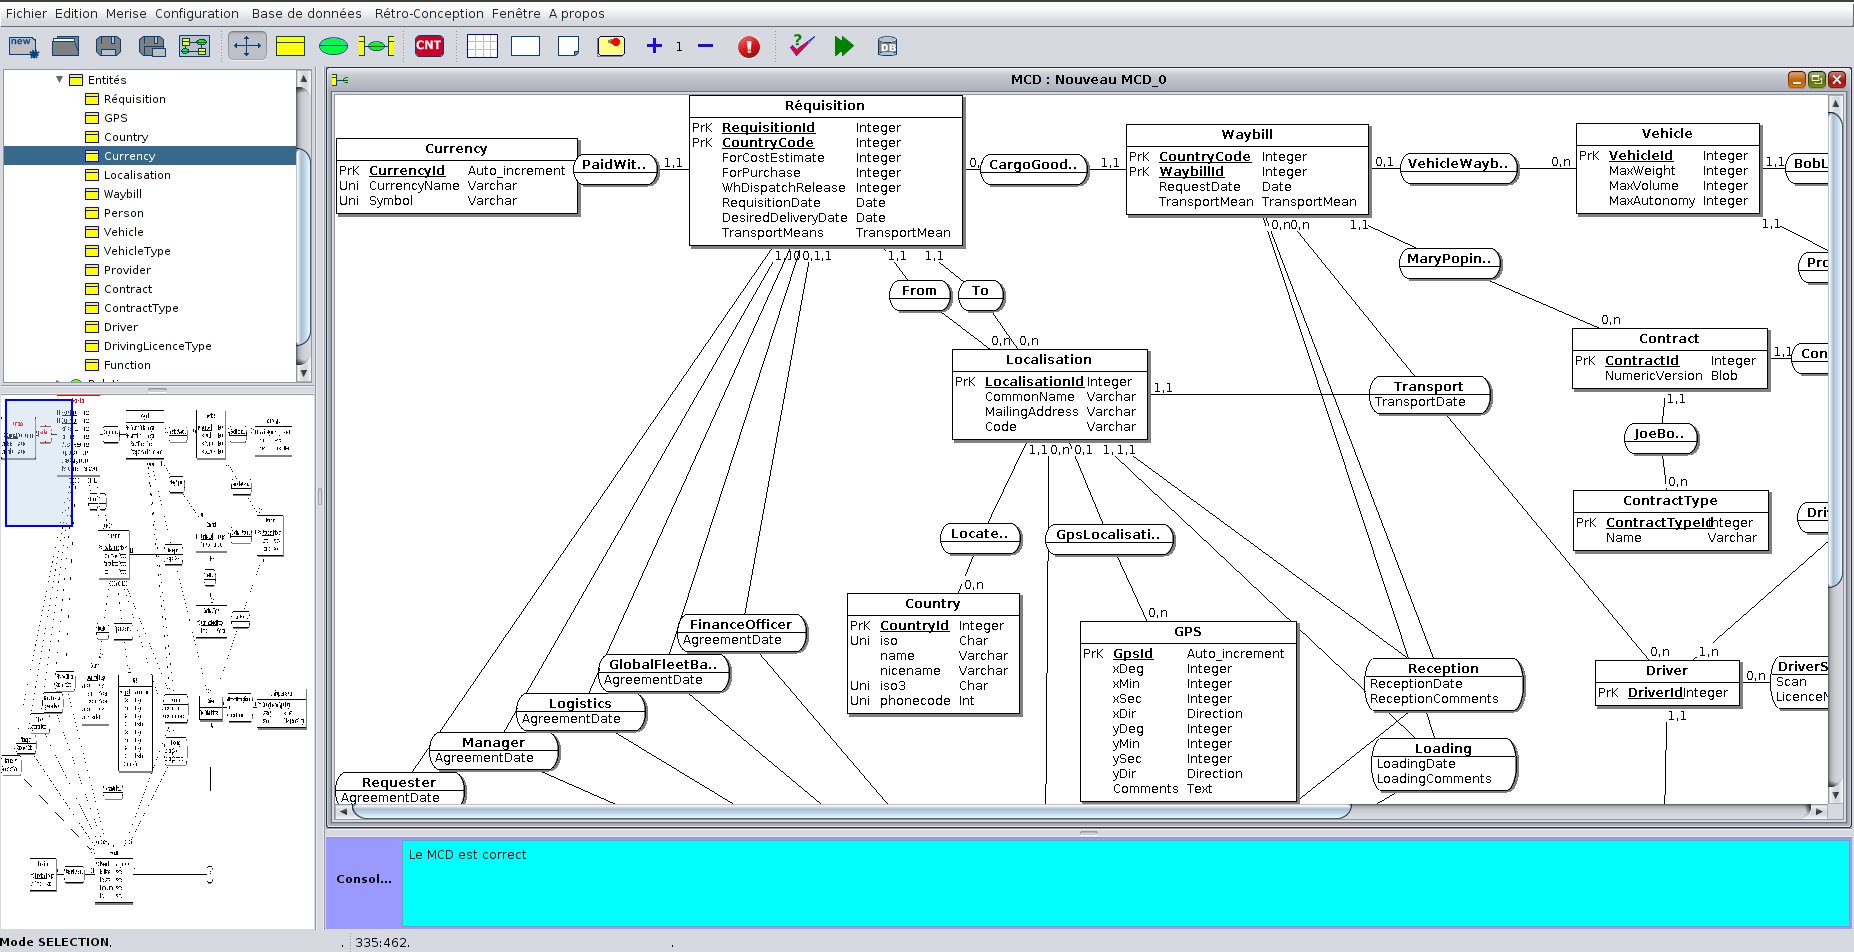
\includegraphics[scale=0.2]{Images/jmerise}
\end{center}

 \subsubsection{Procédure d'installation de JMerise}
Pour installer et utiliser JMerise, dezipper simplement le fichier "\textbf{JMerise.zip}" et exécuter le jar nommé "\textit{JMerise.jar}". 

 \subsubsection{Génération de tables SQL}
Une fois la MCD réalisée à l'aide des outils de conception dans l'onglet "\textit{Merise}", Il est possible de procéder à sa vérification afin de s'assurer que le modèle crée soit correct.
Pour cela, il suffit de cliquer sur le bouton 
\includegraphics[scale=0.35]{checkMCD}.\\\\
L'outil peut aussi générer la MPD associée ainsi que le code SQL sous différents format dont MySQL mais aussi sous forme XML en fournissant la DTD du modèle. Pour cela, il suffit de cliquer sur le bouton 
\includegraphics[scale=0.35]{convertMCD}.\\\\
La suite propose également d'exporter le projet au format \textit{.jpg} ou d'importer un projet tier portant l'extension \textit{.asi}, i.e crée à l'aide du logiciel concurrent \textbf{AnalyseSI}.

 \section{Procédure d'installation de MySQL Server 5.5}
 Ce chapitre décrit la procédure d'installation de MySQL Server 5.5 de Oracle .\\
 La première partie du guide concerne l’installation et l’utilisation de MySQL sur une plateforme Windows.\\
 La seconde, présente la démarche pour installer et utiliser MySQL sur une plateforme Unix.\\
 Enfin, vous pouvez consulter le manuel de référence de MySQL 5.5 qui est disponible 
en ligne sur le site \url{http://dev.mysql.com/doc/refman/5.5/en/}.

 \subsubsection{Installation de MySQL Server 5.5 sous Windows}
 \begin{enumerate}
 \item Aller sur le site \url{https://dev.mysql.com/downloads/installer/5.5.html}
 \begin{figure}
 \centering
 \includegraphics[scale=0.2]{Images/mysqlHomePage}
 \caption{Page de téléchargement de MySQL Server}
 \end{figure}
 \item Sélectionnez la plateforme Microsoft Windows et cliquez sur le bouton Download de la version 
correspondante au système Windows de votre ordinateur, pour télécharger le logiciel dans votre 
ordinateur.
\item On vous propose de vous enregistrer dans le site de MySQL. Si vous avez déjà un nom d’utilisateur, entrez-le, sinon vous pouvez vous enregistrer ou bien vous pouvez continuer le téléchargement sans être enregistré, en cliquant sur la phrase "\textbf{No thanks, just start my download.}"
\item Une fois le téléchargement terminé, double-cliquez sur \textit{mysql-installer-community-MySQL-version.msi} pour lancer l'installateur.\\
 \centering
 \includegraphics[scale=0.5]{Images/mysqlInstaller}
 \item Cliquez sur "\textit{Install MySQL Products}" pour procéder à l'installation de la suite logicielle.
 \item Acceptez le contract de licence en cochant la case "\textit{I accept the licence terms}", puis cliquez sur "\textbf{Next >}"\\
 \centering
 \includegraphics[scale=0.5]{Images/mysqlLicenceAgreement}
 \item Cliquez ensuite sur "\textbf{Execute}" pour vérifier si une nouvelle version du logiciel est disponible ou cocher la case "\textit{Skip the check for updates (not recommended)}" pour passer l'étape de vérification de version.
  \item  Cochez le rond "\textit{Custom}" et cliquez sur "\textbf{Next >}"\\
  \centering
  \includegraphics[scale=0.5]{Images/msqlSetupType}
  \item Sélectionnez la version désirée et vérifié bien que l'architecture est en \textbf{32-Bit}.\\
  \centering
  \includegraphics[scale=0.5]{Images/mysqlVersion}
  \item Cliquez sur "\textbf{Next >}" et "\textbf{Execute}" pour installer les composants de l'application.
  \item Une fois l'installation des composants terminée, cliquez sur "\textbf{Next >}" pour passer à la phase de configuration du server MySQL en trois étapes.\\
  \centering  
  \includegraphics[scale=0.5]{Images/mysqlConfiguration1}
  \item Cliquez sur "\textbf{Next >}" pour passer à l'étape suivante pour définir un mot de passe root pour s'authentifier au server MySQL.\\
 \centering 
 \includegraphics[scale=0.5]{Images/mysqlConfiguration2}
 \item Spécifier un nom de service Windows à utiliser pour cette instance de MySQL Server.\\
 \centering 
 \includegraphics[scale=0.5]{Images/mysqlConfiguration3}
 \item Une fois le server configuré, cliquez sur "\textbf{Next >}" pour lancer la configuration des fichiers exemples fournis dans la suite logicielle, puis cliquez sur "\textbf{Next >}".
 \item Pour terminer l'installation cliquez sur "\textbf{Finish}".\\
 \centering
 \includegraphics[scale=0.5]{Images/mysqlComplete}
 \end{enumerate}
 
 \subsubsection{Utilisation de MySQL Server 5.5 sous Windows}
 Comme nous l'avons vu durant l'installation, MySQL est installé comme un service du système Windows. Cela sous-entend que ce service démarrera à chaque redémarrage de la machine.\\
 Pour définir les options relatives au lancement du service MySQL, ouvrir une console CMD et exécuter la commande suivantes pour ouvrir le gestionnaire de services Windows~:
 \begin{lstlisting}
 > services.msc
 \end{lstlisting}
 \begin{figure}
 \centering
 \includegraphics[scale=0.5]{Images/mysqlServices}
 \caption{Gestionnaire de services Windows}
 \end{figure}
 
 \begin{enumerate}
 \item Pour démarrer votre travail, ouvrez la "\textit{MySQL 5.5 Command Client}"se trouvant dans $C: \backslash Program Files\backslash MySQL \backslash MySQL Server 5.5\backslash bin \backslash$
 Vous allez voir la fenêtre de travail suivante~:\\
 \centering
 \includegraphics[scale=0.6]{Images/mysqlCommandLine}
 \item Entrez votre mot de passe root que vous avez renseigné lors de l'étape d'installation puis appuyer sur la touche \textit{Entrée} du clavier.\\
 \centering
 \includegraphics[scale=0.6]{Images/mysqlCommandLineOk}\\
 Veuillez noter le texte "\textbf{mysql>}" témoignant du changement de contexte du programme MySQL.
 \end{enumerate}
 
 \textbf{Note}
 \begin{itemize}
 \item Les commandes doivent se terminer par le caractère point-virgule ";"
 \end{itemize}

% TODO: A Compléter
 \subsubsection{Installation de MySQL Server 5.5 sous Unix} 

 \subsubsection{Utilisation de MySQL Server 5.5 sous Unix}